\documentclass[a4paper,12pt,reqno]{article}

\newcommand{\CRTdocFormat}{Техническое задание}
\usepackage{styledoc19}

\newcommand{\CRTdocnumMID}{ТЗ 01-1}
\usepackage{CRTconfig}

\begin{document} % конец преамбулы, начало документа
  \CRTpreamble

  \section{Введение}
  \subsection{Наименование программы}
  \subsubsection{Наименование программы на русском языке}
  <<\CRTname>>
  \subsubsection{Наименование программы на английском языке}
  <<\CRTnameeng>>

  \subsection{Краткая характеристика области применения}
  На многих операционных системах редакторы скриншотов отличаются и часто не содержат множество полезных для работы функций.
  Данное приложение решает эту проблему, так как оно является кроссплатформенным и содержит широкий спектр функций.

  \newpage
  \section{Основания для разработки}
  \subsection{Документы, на основании которых ведется разработка}
  Основанием для разработки является учебный план подготовки бакалавров по направлению 09.03.04 <<Программная инженерия>> и утвержденная академическим руководителем тема курсового проекта.

  \subsection{Наименование темы разработки}
  Наименование темы разработки -- <<\CRTname>>

  Программа выполняется в рамках темы курсовой работы в соответствии с учебным планом подготовки бакалавров по направлению 09.03.04 <<Программная инженерия>> Национального исследовательского университета <<Высшая школа экономики>>, факультет компьютерных наук.

  \newpage
  \section{Назначение разработки}
  \subsection{Функциональное назначение}
  Разрабатываемое приложение <<\CRTname>> предназначено для создания снимка экрана рабочей зоны компьютера и для дальнейшей работы и обработки таких снимков с возможностью добавления текста и графических набросков на основе алгоритмов математических кривых Безье.

  \subsection{Эксплуатационное назначение}
  Программа предназначена для бытового пользователя на компьютерах с операционной системой Windows и Linux.

  \newpage
  \section{Требования к программе}
  \subsection{Требования к функциональным характеристикам}
  \subsubsection{Требования к составу выполняемых функций}
  \label{sec:funcs}
  \begin{enumerate}
    \item Создание снимка экрана на Windows и X11.
    \item Возможность перемещать изображение по экрану.
    \item Возможность увеличивать и уменьшать масштаб.
    \item Добавление текста на изображение встроенным растровым шрифтом.
    \item Добавление графических набросков на изображение мышкой.
    \item Сохранение полученного рисунка в файл.
    \item Сохранение полученного рисунка в буфер обмена.
    \item Функция добавления картинок на изображение с помощью перетаскивания.
  \end{enumerate}

  \subsubsection{Требования к интерфейсу}
  \begin{enumerate}
    \item Поле для отображения редактируемого изображения.
    \item Индикатор текущего увеличения и размера изображения.
    \item По клавише быстрого вызова для каждой функции, описанной в \autoref{sec:funcs}.
    \item Обучающая инструкция, в которой написан список всех функций, описанных в \autoref{sec:funcs}.
  \end{enumerate}

  \subsubsection{Требования к организации входных данных}
  На вход должен подаваться снимок экрана из буфера обмена или любое другое изображение из файла.
  \subsubsection{Требования к организации выходных данных}
  На выход программа должна записывать полученный рисунок в файл в формате PNG или в буфер обмена.
  \subsection{Требования к надежности}
  При любом вводе пользователя программа не должна завершаться аварийно.
  При неправильном формате вводимых данных программа должна выводить сообщение с предупреждением о неправильном формате данных.
  \newpage

  \subsection{Условия эксплуатации}
  \subsubsection{Климатические условия}
  Климатические условия эксплуатации, при которых должны обеспечиваться заданные характеристики, должны удовлетворять требованиям, предъявляемым к персональным компьютерам \cite{gostclimate}.
  Персональный компьютер предназначен для работы в закрытом отапливаемом помещении со стабильными климатическими условиями.
  \begin{enumerate}
    \item влажность от 20\% до 70\%;
    \item температура от 5\degree C до 30\degree C;
    \item атмосферное давление --- от 84 до 106,7 кПа (от 630 до 800 мм рт. ст.)
  \end{enumerate}

  \subsubsection{Требования к пользователю}
  \begin{enumerate}
    \item Среднее школьное образование.
    \item Практические навыки работы с пользовательским интерфейсом операционной системы Windows или Linux.
    \item Способность механически взаимодействовать с персональным компьютером и запускать программу.
  \end{enumerate}

  \subsection{Требования к составу и параметру технических средств}
  Для корректной работы приложения необходимо:
  \begin{enumerate}
    \item Процессор архитектуры x86 или x64 с частотой не менее 1 ГГц;
    \item Не менее 2 ГБ ОЗУ;
    \item Не менее 5 МБ свободного места на жестком диске;
    \item Графическое устройство поддерживавшие OpenGL.
  \end{enumerate}

  \subsection{Требования к информационной и программной совместимости}
  Для корректной работы приложения необходимо:
  \begin{enumerate}
    \item Поддержка графических интерфейсов OpenGL или Vulkan;
    \item Одна из нижеперечисленных операционных систем:
    \begin{itemize}
      \item Unix-подобная операционная система с оконной системой X11;
      \item Windows XP или более поздняя версия операционной системы (32-разрядные или 64-разрядные).
    \end{itemize}
  \end{enumerate}

  % \subsection{Требования к маркировке и упаковке}
  % Программа поставляется в виде программного изделия на внешнем носителе информации --
  % компакт диске (CD), на котором должны содержаться программная документация, приложение
  % (исполняемые файлы и прочие необходимые для работы программы файлы) и
  % презентация проекта.
  % Программное изделие должно иметь маркировку с обозначением наименования изделия,
  % темы разработки, фамилии, имени и отчества исполнителя и руководителя разработки, учебной
  % группы и года выпуска изделия.

  \newpage
  \section{Требования к программной документации}
  \subsection{Предварительный состав программной документации}
  \label{sec:doclist}
  В рамках данной работы должна быть разработана следующая программная документация в соответствии и ГОСТ ЕСПД:
  \begin{itemize}
    \item <<\CRTname>>. Техническое задание \cite{gostTZ};
    \item <<\CRTname>>. Программа и методика испытаний \cite{gostPMI};
    \item <<\CRTname>>. Текст программы \cite{gostTP};
    \item <<\CRTname>>. Пояснительная записка \cite{gostPZ};
    \item <<\CRTname>>. Руководство оператора \cite{gostRO};
  \end{itemize}

  \subsection{Специальные требования к программной документации}
  Документы к программе должны быть выполнены в соответствии с ГОСТ 19.106-78 и ГОСТами к каждому виду документа (см. п. \ref{sec:doclist});

  Пояснительная записка должна быть загружена в систему Антиплагиат через LMS <<НИУ ВШЭ>>.

  Документация и программа сдаются в электронном виде в формате .pdf или .docx в архиве формата .zip или .rar;

  За один день до защиты комиссии все материалы курсового проекта:
  \begin{itemize}
    \item техническая документация,
    \item программный проект,
    \item исполняемый файл,
    \item отзыв руководителя,
    \item лист Антиплагиата
  \end{itemize}
  должны быть загружены одним или несколькими архивами в проект дисциплины <<Курсовой проект 2020-2021>> в личном кабинете в информационной образовательной среде LMS (Learning Management System) НИУ ВШЭ.


  \newpage
  \section{Технико-экономические показатели}
  \subsection{Предполагаемая потребность}
  Программа может быть использована в любой сфере, в которой требуется создание и редактирование снимков экранна.
  % \todo{} тут надо написать что на всех системах редакторы скриншотов разные и в половине из них нету некоторых очень необходимых фич \\
  % а на всяких tiling window manager-ах всё совсем плохо\\
  % поэтому моя программа "extensible"{} и её можно запускать с командной строки\\
  % (тут написать надо только первую строчку)
  % Данная программа предназначена для обучения работе методов синтаксического анализа.
  % Может быть использована любыми образовательными программами, а также любым пользователем для самообразования.

  \subsection{Ориентировочная экономическая эффективность}
  Есть несколько критериев, по которым можно сопоставлять данный проект с аналогами:
  \begin{enumerate}
    \item Открытость исходного кода.
    \item Поддержка операционной системы Linux.
    \item Поддержка операционной системы Windows.
    \item Скорость запуска.
    \item Поддержка анимаций.
    \item Масштабирование методом ближайшего соседа.
    \item Взятие снимков экрана.
    \item Понятность интерфейса.
    \item Возможность добавления текста.
    \item Сглаживание движений мышки при рисование.
    \item Возможность использовать буфер обмена.
    \item Возможность отменять сделанные действия.
  \end{enumerate}
  Рассмотрим, как им соответствуют конкуренты. \\
  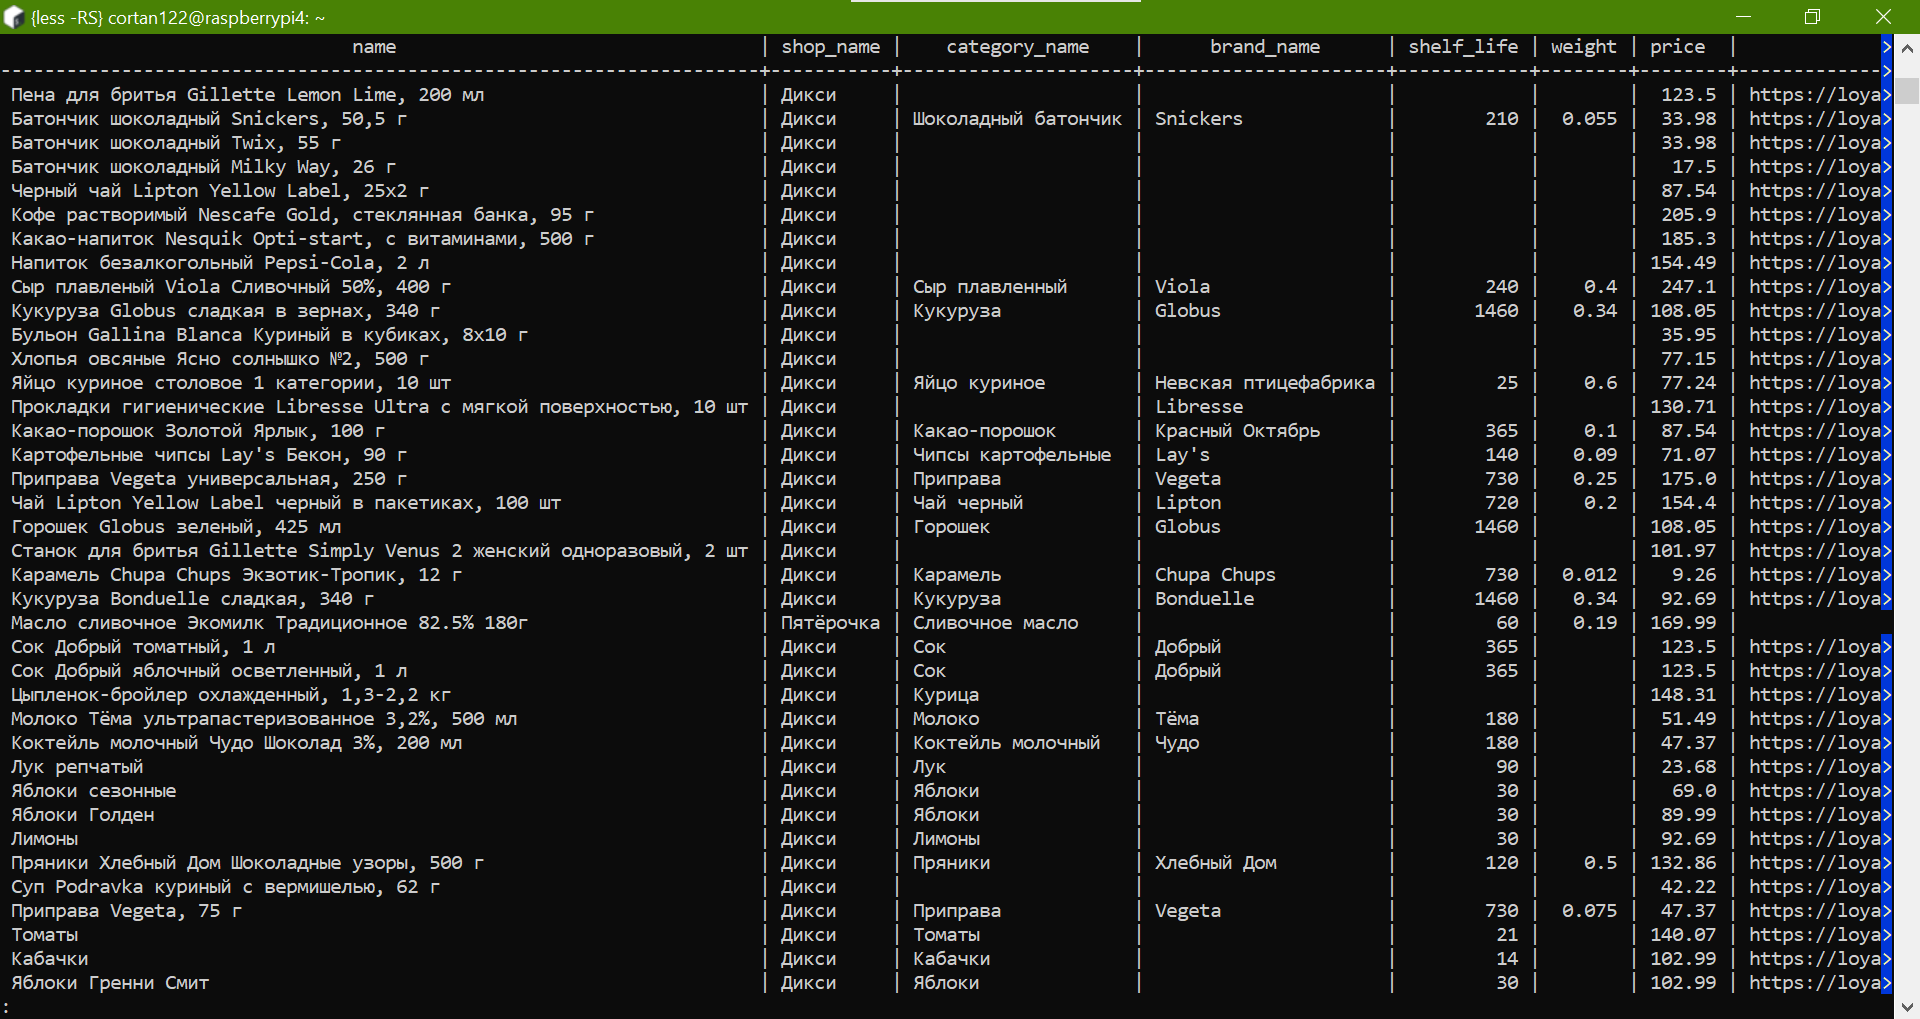
\includegraphics[width=\textwidth]{table.png}
  % \todo{} тут надо написать про анализ аналогов и вставит вот эту табличку \url{https://docs.google.com/spreadsheets/d/1ipV9ayaoG53TJiivB5_lwHFWAxPIj-b-AtXsPpcNKKs}
  % В рамках данной работы расчет экономической эффективности не предусмотрен.

  \newpage
  \section{Стадии и этапы разработки}
    \subsection{Техническое задание}
      \subsubsection*{Обоснование необходимости разработки}
      \begin{enumerate}
        \item Постановка задачи;
        \item Сбор теоретического материала;
        \item Выбор и обоснование критериев эффективности и качества разрабатываемого продукта;
      \end{enumerate}
      \subsubsection*{Научно-исследовательские работы}
      \begin{enumerate}
        \item Определение структуры входных и выходных данных;
        \item Предварительный выбор методов решения поставленной задачи;
        \item Определение требований к техническим средствам;
        \item Обоснование возможности решения поставленной задачи.
      \end{enumerate}
      \subsubsection*{Разработка и утверждение технического задания}
      \begin{enumerate}
        \item Определение требований к программе;
        \item Определение стадий, этапов и сроков разработки программы и документации на неё;
        \item Выбор языка программирования;
        \item Согласование и утверждение технического задания.
      \end{enumerate}
      \subsubsection*{Подготовка и передача программы}
      \begin{enumerate}
        \item утверждение даты защиты программного продукта;
        \item подготовка программы и программной документации для презентации и защиты;
        \item представление разработанного программного продукта руководителю и получение отзыва;
        \item загрузка Пояснительной записки в систему Антиплагиат через ЛМС НИУ ВШЭ;
        \item загрузка материалов курсового проекта (курсовой работы) в ЛМС, проект дисциплины <<Курсовая работа 2020>> (п. 5.2);
        \item Защита программного продукта (курсового проекта) комиссии.
      \end{enumerate}
    \subsection{Рабочий проект}
      \subsubsection*{Разработка программы}
      \begin{enumerate}
        \item Анализ аналогов;
        \item Реализация алгоритма кривых Безье;
        % \item \todo
        \item Реализация программного интерфейса;
        \item Отладка программы.
      \end{enumerate}
      \subsubsection*{Разработка программной документации}
      \begin{enumerate}
        \item Разработка программных документов в соответствии с требованиями ЕСПД.
      \end{enumerate}
      \subsubsection*{Испытания программы}
      \begin{enumerate}
        \item Разработка, согласование и утверждение программы и методики испытаний;
        \item Проведение предварительных приемо-сдаточных испытаний;
        \item Корректировка программы и программной документации по результатам испытаний.
      \end{enumerate}
      \subsubsection*{Сроки разработки и исполнители}
      Разработка должна закончиться к 13 мая 2021 года.

      Исполнитель: AAAAAAA AAAAAAAAAA AAAAAAAAAA, студент группы AAAAAA факультета компьютерных наук НИУ ВШЭ.
    \subsection{Внедрение}
      \subsubsection*{Подготовка и защита программного продукта}
      \begin{enumerate}
        \item Подготовка программы и документации для защиты;
        \item Утверждение дня защиты программы;
        \item Презентация разработанного программного продукта;
        \item Передача программы и программной документации в архив НИУ ВШЭ.
      \end{enumerate}

  % приложения нумеруются отдельно и надо выровнять по правому краю

  % \newpage
  % \addition{Используемые понятия и определения}
  % \todo
  % \newpage

  % \addition{Иллюстрации интерфейса} \label{interface}
  % \todo.

  \section{Порядок контроля и приемки}
  Проверка программного продукта, в том числе и на соответствие техническому заданию,
  осуществляется исполнителем вместе с заказчиком согласно <<Программе и методике испытаний>>, а также пункту 5.2.
  Защита выполненного проекта осуществляется комиссии, состоящей из преподавателей департамента программной инженерии,
  в утверждённые приказом декана ФКН сроки.

  \begin{CRTbibliography}
  \end{CRTbibliography}

  \CRTlistRegistration
\end{document} % конец документа
